\documentclass{bioinfo}
\copyrightyear{2017} \pubyear{2017}

\access{Advance Access Publication Date: Day Month Year}
\appnotes{Application Note}

\begin{document}
\firstpage{1}

\subtitle{Systems Biology}

\title[PyBEL]{PyBEL: a Computational Framework for Biological Expression Language}
\author[Hoyt \textit{et~al}.]{Charles Tapley Hoyt\,$^{\text{\sfb 1,2,*}}$, Andrej Konotopez\,$^{\text{\sfb 1}}$, and Christian Ebeling\,$^{\text{\sfb 1}}$}
\address{$^{\text{\sf 1}}$Department of Bioinformatics, Fraunhofer Institute for Algorithms and Scientific Computing (SCAI), Sankt Augustin, 53754, Germany \\
$^{\text{\sf 2}}$Bonn-Aachen International Center for IT, Rheinische Friedrich-Wilhelms-Universit{\"a}t Bonn, Bonn, 53113, Germany.}

\corresp{$^\ast$To whom correspondence should be addressed.}
\history{Received on XXXXX; revised on XXXXX; accepted on XXXXX}
\editor{Associate Editor: XXXXXXX}

\abstract{\textbf{Summary:} Biological Expression Language (BEL) assembles knowledge networks from biological relations across multiple modes and scales. Here, we present PyBEL; a software package for parsing, validating, converting, storing, querying, and visualizing networks encoded in BEL.\\
\textbf{Availability:}  PyBEL is implemented in platform-independent, universal Python code. Its source is distributed under the Apache 2.0 License at https://github.com/pybel.\\
\textbf{Contact:} \href{charles.hoyt@scai.fraunhofer.de}{charles.hoyt@scai.fraunhofer.de}\\
\textbf{Supplementary information:} Supplementary data are available at \textit{Bioinformatics} online.}

\maketitle

\section{Introduction}

Among the most popular modeling and data exchange languages in systems biology are currently the Biological Pathways Exchange (BioPAX), Systems Biology Markup Language (SBML), and Biological Expression Language (BEL). BioPAX captures metabolic, signaling, molecular, gene-regulatory, and genetic interaction networks (\citealp{Hucka2013}); SBML accommodates mathematical models of biochemical networks, cellular signaling, and metabolic pathways (\citealp{Demir2010}); and BEL assembles qualitative causal and correlative relations between biological entities across multiple modes and scales, with full provenance information including namespace references, relation provenance (citation and evidence), and biological context-specific relation metadata (anatomy, cell, disease, etc.) (\citealp{Slater2014}).

While there exist several software packages for BioPAX and SBML, the ecosystem of open-source software for BEL is much more limited. An assessment of previous software (see \textbf{Table 3} of the supplementary information) shows there is an unmet need for easily installable, stable, facile software that parses modern BEL and provides programmatic access to a data container that enables the resulting network to be extended, queried, manipulated, analyzed, and visualized. Furthermore, a converter between common data formats is needed to enable re-usability and interoperability between general and BEL-specific software for network analysis and visualization. 

Here, we present PyBEL; a software package designed to fulfill each of these needs. 

\section{Software Architecture}

The PyBEL software package consists of five main components: (1) network data container, (2) parser and validator, (3) network database manager, (4) data converter, and (5) network visualizer. 

While a graph refers to an abstraction for a set of objects (i.e.\ nodes) and their relations (i.e.\ edges), its instantiation in a real-world application is often called a network. We provide an implementation of a directed multigraph (i.e.\ a graph whose edges have directionality and any given pair of nodes may have multiple edges) that maps the biological entities and concepts in the subjects and objects of BEL relations to nodes in a network and their relations, with corresponding metadata, to edges. We extended the MultiDiGraph class from \verb|NetworkX| (http://networkx.github.io) to enable users direct access to their suite of network algorithms and static visualizations to support their further development into biologically meaningful analyses.

The parser performs tokenization, lexical analysis, parsing, and validation on each of the three sections of BEL documents (see \textbf{Figures 1 and 2} of the supplementary information). Callbacks are used to annotate the entries in the document metadata section to a network instance, download and store the resources referenced in the definitions section, maintain a list of current annotations from \verb|SET| statements, and parse BEL relations to populate a network instance with the corresponding nodes, edges, and their metadata from the current internal state. While relations' syntax is implicitly validated, the semantics of their subjects' and objects' identifiers are validated against the references from the definitions section. Finally, feedback is provided to users to support thoughtful re-curation, which could lead to more robust knowledge assemblies and enable more reproducible science.

Namespaces and networks are cached with a relational database to improve the speed of validation and access to data. While relational databases lack the faculty for applying network algorithms, they provide indexing functionality that enables complicated queries and filters over the nodes, edges, and metadata of increasingly large collections of networks. For example, this could help identify intersections and potential cross-talk between disease-specific networks. 

We implemented lossless converters for common file formats including Node-Link JSON, JGIF, CX, and binary as well as for database formats including SQL, Neo4J, and NDEx. We also provide lossy exporters to Excel, CSV, SIF, XGMML, and GSEA to facilitate usage in other programs. Notably, we have deferred implementing a RDF (Resource Description Framework) converter until improvements are made to the existing BEL to RDF mapping and its documentation (https://wiki.openbel.org). Future work will also include converters for BioPAX and SBML. See \textbf{Tables 1-2} of the supplementary information for more detailed descriptions of each format.  

Networks can be exported for visualization in Cytoscape or uploaded to NDEx (\citealp{Pratt2015}) to take advantage of its viewer and simple query interface. Alternatively, we provide an interactive network explorer tailored to BEL networks (appropriate node coloring, metadata pop-ups, etc.) that can be directly embedded as HTML in email, Jupyter Notebook, or a web application. It has already been used to produce visualizations in the NeuroMMSig Web Service (\citealp{Domingo-Fernandez2017}). \textbf{Figures 3-5} of the supplementary information present these visualizations side-by-side. In addition to their programmatic interfaces, the parser, storage, conversion, and visualization features are exposed via a command line tool.

\section{Case Study}

The PyBEL suite includes functions for querying and mutating networks with which it implements state-of-the-art algorithms for over-representation analysis, functional class scoring, and pathway topological analysis of BEL networks such as Reverse Causal Reasoning (\citealp{Catlett2013}). \textbf{Figure 1} presents a case study in which a novel heat diffusion work flow was used to assess the observed impact on biological processes from differential gene expression in Alzheimer's disease (AD). Technical documentation is included in the supplementary information.

\begin{figure}[!tpb]%figure2
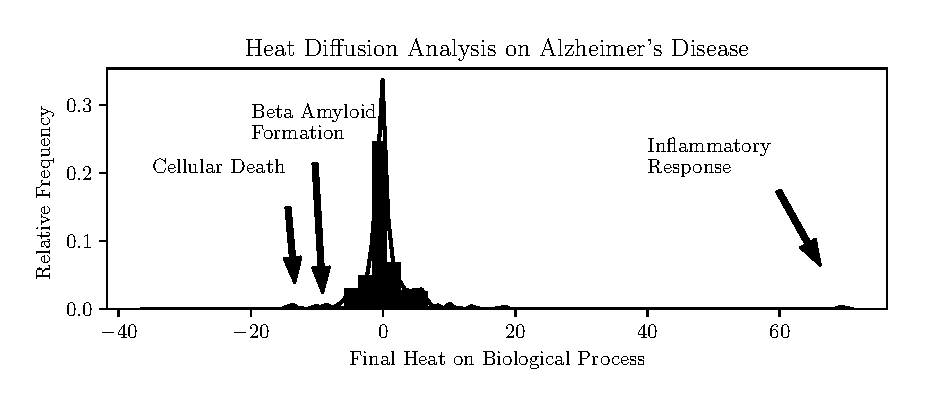
\includegraphics[width=8cm]{figure1.eps}
\caption{Plotted is the distribution of the final heat on biological processes from the NeuroMMSig AD Knowledge Assembly (\citealp{Domingo-Fernandez2017}) following heat diffusion analysis with a differential gene expression experiment from the brains of AD patients (E-GEOD-5281, \citealp{Liang2007}). The significant down-regulation of biological processes related to inflammatory response (heat=69) and up-regulation of cellular death (heat=-13) and beta-amyloid formation (heat=-9) match common clinical observations and serve as a validation for this approach.}\label{fig:01}
\end{figure}

\section{Discussion}

Even after its v2.0 update, BEL does not yet explicitly specify many concepts in molecular biology such as epigenetic information (\citealp{Irin2015}). The inevitability of language evolution prompted us to develop the parser in modules so that new syntax could be proposed and implemented quickly. As a proof of concept, a syntax extension for gene modifications is included in the package by default.

Historically, BEL has used a custom namespace file format, but the creation and maintenance of biological terminologies has tended towards using OWL (Web Ontology Language). Furthermore, many domains (e.g.\ SNPs) are growing too large to enumerate during semantic integration and validation. The modular architecture of the parser enables easy implementation of new definition file formats, external validation services, or even alternative namespace definition schemes to address these issues.

While BEL is often used to formalize knowledge curated from unstructured sources, our software also enables the integration of knowledge from structured sources. For example, existing solutions for resolving equivalences across namespaces rely on the creation and hosting of extensive lookup tables. Alternatively, the parser could be extended with a dedicated syntax and draw equivalencies directly from OWL.

Finally, we plan to present this software as a web service to enable a wider audience of researchers across disciplines to validate, explore, and analyze their BEL networks.

\section*{Acknowledgements}

We thank Sumit Madan and Scott Colby for their advice and feedback.

\section*{Funding}

This work was supported by the EU/EFPIA Innovative Medicines Initiative Joint Undertaking under AETIONOMY [grant number 115568], resources of which are composed of financial contribution from the European Union's Seventh Framework Programme (FP7/2007-2013) and EFPIA companies in kind contribution.

Conflict of Interest: none declared.

\begin{thebibliography}{}

\bibitem[Catlett \textit{et~al}., 2013]{Catlett2013}
Catlett, N., et al. (2013). Reverse causal reasoning: applying qualitative causal knowledge to the interpretation of high-throughput data. BMC Bioinformatics, 14(1), 340.

\bibitem[Demir \textit{et~al}., 2010]{Demir2010}
Demir, E., et al. (2010). The BioPAX community standard for pathway data sharing. Nature Biotechnology, 28(12), 1308-1308.

\bibitem[Domingo-Fern\'{a}ndez \textit{et~al}., 2017]{Domingo-Fernandez2017}
Domingo-Fern\'{a}ndez, D., et al. (2017). Multimodal Mechanistic Signatures for Neurodegenerative Diseases (NeuroMMSig): a web server for mechanism enrichment. Bioinformatics (Oxford, England), btx399.

\bibitem[Hucka \textit{et~al}., 2013]{Hucka2013}
Hucka, M., et al. (2003). The systems biology markup language (SBML): a medium for representation and exchange of biochemical network models. Bioinformatics (Oxford, England), 19(4), 524-531.

\bibitem[Irin \textit{et~al}., 2015]{Irin2015}
Irin, A. K., et al. (2015). Computational Modelling Approaches on Epigenetic Factors in Neurodegenerative and Autoimmune Diseases and Their Mechanistic Analysis. Journal of Immunology Research, 2015.

\bibitem[Liang \textit{et~al}., 2007]{Liang2007}
Liang, W. S., et al.. (2007). Gene expression profiles in anatomically and functionally distinct regions of the normal aged human brain. Physiological Genomics, 28(3), 311-322.

\bibitem[Pratt \textit{et~al}., 2015]{Pratt2015}
Pratt, D., et al. (2015). NDEx, the Network Data Exchange. Cell Systems, 1(4), 302-305.

\bibitem[Slater, 2014]{Slater2014}
Slater, T. (2014). Recent advances in modeling languages for pathway maps and computable biological networks. Drug Discovery Today, 19(2), 193-198.

\end{thebibliography}
\end{document}
